\documentclass{article}\usepackage[]{graphicx}\usepackage[]{color}
%% maxwidth is the original width if it is less than linewidth
%% otherwise use linewidth (to make sure the graphics do not exceed the margin)
\makeatletter
\def\maxwidth{ %
  \ifdim\Gin@nat@width>\linewidth
    \linewidth
  \else
    \Gin@nat@width
  \fi
}
\makeatother

\definecolor{fgcolor}{rgb}{0.345, 0.345, 0.345}
\newcommand{\hlnum}[1]{\textcolor[rgb]{0.686,0.059,0.569}{#1}}%
\newcommand{\hlstr}[1]{\textcolor[rgb]{0.192,0.494,0.8}{#1}}%
\newcommand{\hlcom}[1]{\textcolor[rgb]{0.678,0.584,0.686}{\textit{#1}}}%
\newcommand{\hlopt}[1]{\textcolor[rgb]{0,0,0}{#1}}%
\newcommand{\hlstd}[1]{\textcolor[rgb]{0.345,0.345,0.345}{#1}}%
\newcommand{\hlkwa}[1]{\textcolor[rgb]{0.161,0.373,0.58}{\textbf{#1}}}%
\newcommand{\hlkwb}[1]{\textcolor[rgb]{0.69,0.353,0.396}{#1}}%
\newcommand{\hlkwc}[1]{\textcolor[rgb]{0.333,0.667,0.333}{#1}}%
\newcommand{\hlkwd}[1]{\textcolor[rgb]{0.737,0.353,0.396}{\textbf{#1}}}%
\let\hlipl\hlkwb

\usepackage{framed}
\makeatletter
\newenvironment{kframe}{%
 \def\at@end@of@kframe{}%
 \ifinner\ifhmode%
  \def\at@end@of@kframe{\end{minipage}}%
  \begin{minipage}{\columnwidth}%
 \fi\fi%
 \def\FrameCommand##1{\hskip\@totalleftmargin \hskip-\fboxsep
 \colorbox{shadecolor}{##1}\hskip-\fboxsep
     % There is no \\@totalrightmargin, so:
     \hskip-\linewidth \hskip-\@totalleftmargin \hskip\columnwidth}%
 \MakeFramed {\advance\hsize-\width
   \@totalleftmargin\z@ \linewidth\hsize
   \@setminipage}}%
 {\par\unskip\endMakeFramed%
 \at@end@of@kframe}
\makeatother

\definecolor{shadecolor}{rgb}{.97, .97, .97}
\definecolor{messagecolor}{rgb}{0, 0, 0}
\definecolor{warningcolor}{rgb}{1, 0, 1}
\definecolor{errorcolor}{rgb}{1, 0, 0}
\newenvironment{knitrout}{}{} % an empty environment to be redefined in TeX

\usepackage{alltt}

\usepackage{fancyhdr} % Required for custom headers
\usepackage{lastpage} % Required to determine the last page for the footer
\usepackage{extramarks} % Required for headers and footers
\usepackage{graphicx} % Required to insert images
\usepackage{hyperref}
\usepackage{amsmath} %for binomial pdf
\usepackage{parskip} % so that there's space bw paragraphs
\usepackage{float}
\usepackage{amsfonts}

% Margins
\topmargin=-0.45in
\evensidemargin=0in
\oddsidemargin=0in
\textwidth=6.5in
\textheight=9.0in
\headsep=0.25in 

\linespread{1.1} % Line spacing

% Set up the header and footer
\pagestyle{fancy}
\lhead{STAT 534: Spatial} % Top left header
\chead{HW 1} % Top center header
\rhead{Andrea Mack} % Top right header
\lfoot{01/18/2017} % Bottom left footer
\cfoot{} % Bottom center footer
\rfoot{Page\ \thepage\ of\ \pageref{LastPage}} % Bottom right footer
\renewcommand\headrulewidth{0.4pt} % Size of the header rule
\renewcommand\footrulewidth{0.4pt} % Size of the footer rule

\setlength\parindent{0pt} % Removes all indentation from paragraphs
\setlength\parskip{0.5cm}
\restylefloat{table}

%----------------------------------------------------------------------------------------
%	DOCUMENT STRUCTURE COMMANDS
%	Skip this unless you know what you're doing
%----------------------------------------------------------------------------------------

% Header and footer for when a page split occurs within a problem environment
\newcommand{\enterProblemHeader}[1]{
\nobreak\extramarks{#1}{#1 continued on next page\ldots}\nobreak
\nobreak\extramarks{#1 (continued)}{#1 continued on next page\ldots}\nobreak
}

% Header and footer for when a page split occurs between problem environments
\newcommand{\exitProblemHeader}[1]{
\nobreak\extramarks{#1 (continued)}{#1 continued on next page\ldots}\nobreak
\nobreak\extramarks{#1}{}\nobreak
}


%----------------------------------------------------------------------------------------%
\IfFileExists{upquote.sty}{\usepackage{upquote}}{}
\begin{document}



\begin{enumerate}
\item {\it Our text implies and others state outright that the BB, BW , and WW statistics reveal pretty much the same thing about spatial correlation. The joincount.mc function will carry out Monte Carlo tests based on the BB and WW statistics. We do not have an R formula for computing the BW statistic but it is possible to carry out a BW joincount test of spatial autocorrelation (or clustering) using Geary’s c.}

\begin{enumerate}
\item {\it Show the relationship between Geary’s c and BW.}
\vspace{3in}

\item {\it Carry out a test based on the BW statistics using geary.mc. The data file atrplx.dat will be emailed to you at your math department email addresses. The first 2 columns contain the spatial coordinates and the fourth column contains the Z values you need. Use the R handout to generate the necessary neighbors and list objects.}

All tests are done using the one sided alternative.

Let c = Geary's C statistic, which is a measure of similarity in responses, accounting for spatial proximity

$H_{0}$: c = E[c] = no spatial autocorrelation (random pattern)

$H_{A}$: c \textless E[c] = positive spatial autocorrelation (positive non-random pattern, positive systematic pattern)

Note the alternative makes sense because in (a) we showed that Geary's c is equivalent to computing a BW statistic, which measures the number of BW connections. The fewer BW connections, the more BB/WW connections, indicating more similar responses at closer locations and is why the sign is opposite. 

1000 Monte Carlo simulations led to a p-value of 0.127 using an observed Geary's C of 0.95. There is no evidence of a positive spatial autocorrelation in the responses. 





\begin{knitrout}\footnotesize
\definecolor{shadecolor}{rgb}{0.969, 0.969, 0.969}\color{fgcolor}\begin{kframe}
\begin{verbatim}

	Monte-Carlo simulation of Geary C

data:  atrplx$z 
weights: atrplx_w 
number of simulations + 1: 1000 

statistic = 0.94756, observed rank = 131.5, p-value = 0.1315
alternative hypothesis: greater
\end{verbatim}
\end{kframe}

{\centering 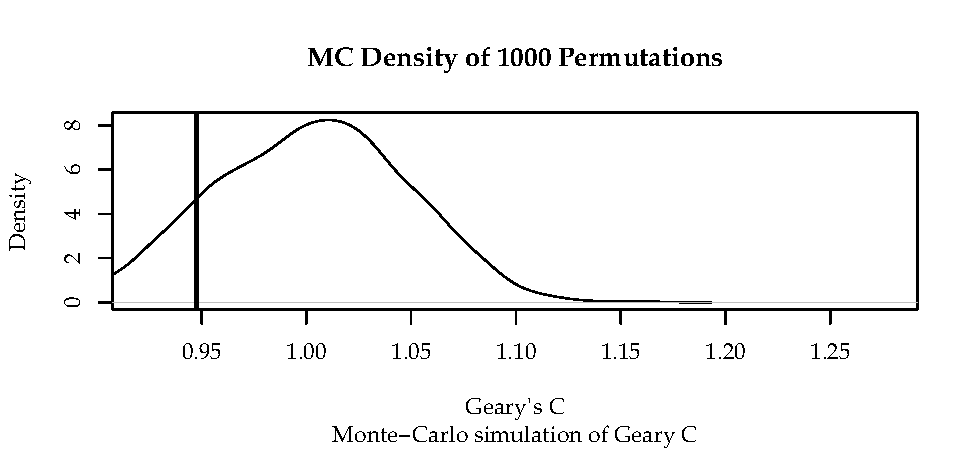
\includegraphics[width=\maxwidth]{figure/prob1b_out-1} 

}



\end{knitrout}

\item %1c
{\it Using the output from geary.mc compute BW and E[BW]. Do you expect BW \textless E[BW] or BW \textgreater E[BW] in the presence of positive spatial clustering of the plants? Why or why not?}



In the prescense of positive spatial clustering of plants I would expect BW \textless E[BW]. More B-W joins suggests fewer similar plants (meaning B-B or W-W) clustered. Positive spatial clustering of plants occurs when similar plants (B-B or W-W) are located closer together, thereby fewer dis-similar plants (B-W) being located closer together.

The output from {\texttt geary.mc} resulted in a test statistic of 0.948, leading to a BW test statistic of 173. 

E[BW] = $\pi(1-\pi)*\Sigma_{i}\Sigma_{j}w_{ij}$ where $w_{ij}$ = $w_{\cdot\cdot}$

Using non-free sampling, E[BW] = 0.254*0.746*960 = 181.86.

BW is less than E[BW] under no spatial autocorrelation and aligns with what was proposed above given there was no evidence of spatial autocorrelation.



\item %1d
{\it Reproduce the analysis I presented in class using the Atriplex data. Compare the results of the BW test to those of the BB and WW test that were discussed in class. Do these statistics all seem to indicate the same thing about spatial clustering of the plants.}

The three tests do not all result in the same conclusion. Using the BW (c) statistic and the WW statistic, there is no evidence of positive spatial clustering (p-values of 0.125 and 0.414, respectively), though the magnitudes of the p-values differ quite a bit. Using the BB statistic, with a p-value of 0.02 there is strong evidence of positive spatial clustering.  


\newpage

\item %1e

{\it  For grins compute Moran’s I and compare that result to those above.}

\begin{knitrout}\footnotesize
\definecolor{shadecolor}{rgb}{0.969, 0.969, 0.969}\color{fgcolor}\begin{kframe}
\begin{verbatim}

	Monte-Carlo simulation of Moran I

data:  atrplx$z 
weights: atrplx_w  
number of simulations + 1: 1000 

statistic = 0.068342, observed rank = 943, p-value = 0.057
alternative hypothesis: greater
\end{verbatim}
\end{kframe}
\end{knitrout}

Using Moran's I, there is some evidence of positive spatial autocorrelation with a p-value of 0.057, which falls between the amount of evidence for spatial autocorrelation found using Geary's C (BW) and the BB tests.


\end{enumerate}

\item {\it Categorize the following examples of spatial data as to their data type:}
\begin{enumerate}
\item %2a 
{\it Elevations in the foothills of the Allegheny mountains.}

Geostatistical

\item %2b
{\it Highest elevation within each state in the United States.}

Lattice

\item %2c
{\it Concentration of a mineral in soil.}

Geostatistical

\item %2d
{\it Plot yields in a uniformity trial.}

Lattice

\item %2e
{\it Crime statistics giving names of subdivisions where break-ins occurred in the previous year and property loss values.}

Point process

\item %2f
{\it Same as previous, but instead of the subdivisions, the individual dwelling, is identified.}

Point process

\item %2g
{\it Distribution of oaks and pines in a forest stand.}

Point process
%Geostatistical
\end{enumerate}
\newpage

\item %3
{\it Show that Moran’s I is a scale-free statistic, i.e. Z(s) and $\lambda$ Z(s) yield the same value for any constant $\lambda \neq$ 0.}
\vspace{4in}

\item %4

\begin{enumerate}
\item %4a
{\it Show the $Var(\bar{Y})$ = }

\vspace{4in}

\item %4b
{\it Let n = 10 and ρ = 0.26. Compare and contrast a 95\% confidence interval for $\mu$ computed using the true standard deviation of Y and one computed assuming independence.}

With n = 10 and $\rho$ = 0.26, a 95\% confidence interval accounting for the spatial correlation structure will be about twice the width of that found assuming independence. However, both have the same center and the same multiplier.


{\bf Assuming Independence:}


$\bar{y} \pm 1.96(\frac{\sigma^{2}}{10})^{1/2}$


= $\bar{y} \pm 0.62\sigma$


{\bf Assuming Correlated:}


$\bar{y} \pm 1.96(\frac{\sigma^{2}}{n}[1+(n-1)\rho])^{1/2})$


= $\bar{y} \pm 1.96(\frac{\sigma^{2}}{10}[1+(10-1)*0.26])^{1/2})$


= $\bar{y} \pm 1.13*\sigma$


\item %4c 

{\it Given independence, we know that Y is the ``best" estimator of $\mu$. One nice property it has is that it is a consistent estimator of the mean. Is Y a consistent estimator of the mean given the correlation structure above? Justify your answer.}
\vspace{4in}

\newpage
\item %4d
{\it Recall that effective sample size is a measure of the effect of correlation on inference. An equation for the effective sample size under the equicorrelation model is:}
\begin{center}
$n^{'} = \frac{n}{1+(n-1)\rho}$
\end{center}


{\it The effective sample size is defined to be the sample size $n^{'}$ of uncorrelated observations that provide the same information (in a sense) as a sample of n correlated observations.}

\begin{enumerate}
\item %4di

{\it Compute the effective sample size when n = 10, 100, and 1000 and $\rho$ = 0.05, 0.1, 0.25, and 0.5.}

% latex table generated in R 3.3.2 by xtable 1.8-2 package
% Wed Jan 18 10:20:20 2017
\begin{table}[ht]
\centering
\begin{tabular}{||l|l|l|l|l||}
  \hline
 & rho0.05 & rho0.1 & rho0.25 & rho0.5 \\ 
  \hline
n10 & 6.90 & 5.26 & 3.08 & 1.82 \\ 
  n100 & 16.81 & 9.17 & 3.88 & 1.98 \\ 
  n1000 & 19.63 & 9.91 & 3.99 & 2.00 \\ 
   \hline
\end{tabular}
\end{table}


\item %4dii
{\it Find lim $n^{'}$ as n $\rightarrow$ infinite.}

\vspace{3in}

\item %4diii

{\it The effect is extreme here but we would not expect to see this type of correlation structure in a spatial setting. Why not?}

We would not expect the equicorrelation structure in a spatial setting because the equicorrelation structure would assume that points are equally correlated, regardless of the distance between them. One of the major aspects of spatial data is that observations in closer proximity to each other tend to have more similar responses, which is not accounted for in the equicorrelation structure.

\end{enumerate}
\end{enumerate}

\end{enumerate}

\newpage

\section*{R Code}
\begin{knitrout}\footnotesize
\definecolor{shadecolor}{rgb}{0.969, 0.969, 0.969}\color{fgcolor}\begin{kframe}
\begin{alltt}
\hlcom{#first compute number of "distance based" neighbors (vs. color based)}
\hlcom{#using lower and upper distance bounds from notes}
\hlstd{atrplx_nn} \hlkwb{<-} \hlkwd{dnearneigh}\hlstd{(}\hlkwd{as.matrix}\hlstd{(atrplx[,}\hlkwd{c}\hlstd{(}\hlnum{1}\hlstd{,}\hlnum{2}\hlstd{)]),} \hlkwc{d1} \hlstd{=} \hlnum{0}\hlstd{,} \hlkwc{d2} \hlstd{=} \hlnum{1}\hlstd{)}
\hlkwd{card}\hlstd{(atrplx_nn)}

\hlcom{#calculate spatial weights -> "B" = binary}
\hlstd{atrplx_w} \hlkwb{<-} \hlkwd{nb2listw}\hlstd{(atrplx_nn,} \hlkwc{style} \hlstd{=} \hlstr{"B"}\hlstd{)}
\end{alltt}
\end{kframe}
\end{knitrout}
\begin{knitrout}\footnotesize
\definecolor{shadecolor}{rgb}{0.969, 0.969, 0.969}\color{fgcolor}\begin{kframe}
\begin{alltt}
\hlcom{#do monte carlo simulation based test}
\hlstd{gc.out} \hlkwb{<-} \hlkwd{geary.mc}\hlstd{(atrplx}\hlopt{$}\hlstd{z,atrplx_w,} \hlkwc{nsim} \hlstd{=} \hlnum{999}\hlstd{)}

\hlstd{gc.out}

\hlcom{# randomly shuffles response and re-assigns to atrplx_w 1000 times}
\hlcom{# calculate geary's c for each shuffle}
\hlcom{# plot the shuffled geary's c's and find the rank of that observed}

\hlkwd{plot}\hlstd{(gc.out,} \hlkwc{main} \hlstd{=} \hlstr{"MC Density of 1000 Permutations"}\hlstd{,} \hlkwc{xlab} \hlstd{=} \hlstr{"Geary's C"}\hlstd{)}
\end{alltt}
\end{kframe}
\end{knitrout}
\begin{knitrout}\footnotesize
\definecolor{shadecolor}{rgb}{0.969, 0.969, 0.969}\color{fgcolor}\begin{kframe}
\begin{alltt}
\hlcom{# computing the BW statistic using (a) and (b)}

\hlcom{#note third column has BW coding}

\hlcom{# the output of the dnearneigh() object gives the total number}
\hlcom{# of non-zero joints in the distance matrix, which is w_dot,dot}

\hlstd{w2dot} \hlkwb{<-} \hlnum{960}
\hlstd{z_mean} \hlkwb{<-} \hlkwd{mean}\hlstd{(atrplx[,}\hlnum{4}\hlstd{])}

\hlstd{s2} \hlkwb{<-} \hlstd{(}\hlkwd{sum}\hlstd{((atrplx[,}\hlnum{4}\hlstd{]} \hlopt{-} \hlstd{z_mean)}\hlopt{^}\hlnum{2}\hlstd{))}\hlopt{/}\hlstd{(}\hlkwd{dim}\hlstd{(atrplx)[}\hlnum{1}\hlstd{]} \hlopt{-} \hlnum{1}\hlstd{)}

\hlcom{# from (a), get to BW from c by multiplying c by s2*w2dot}

\hlstd{bw} \hlkwb{<-} \hlstd{gc.out}\hlopt{$}\hlstd{statistic}\hlopt{*}\hlstd{s2}\hlopt{*}\hlstd{w2dot}

\hlcom{# use the observed proportion of blacks = n1 -> non-free sampling}
\hlstd{pi} \hlkwb{<-} \hlkwd{sum}\hlstd{(atrplx[,}\hlnum{4}\hlstd{])}\hlopt{/}\hlkwd{dim}\hlstd{(atrplx)[}\hlnum{1}\hlstd{]}

\hlstd{e_bw} \hlkwb{<-} \hlstd{pi}\hlopt{*}\hlstd{(}\hlnum{1}\hlopt{-}\hlstd{pi)}\hlopt{*}\hlstd{w2dot}
\end{alltt}
\end{kframe}
\end{knitrout}
\begin{knitrout}\footnotesize
\definecolor{shadecolor}{rgb}{0.969, 0.969, 0.969}\color{fgcolor}\begin{kframe}
\begin{alltt}
\hlstd{gc.out_mean} \hlkwb{<-} \hlkwd{mean}\hlstd{(gc.out}\hlopt{$}\hlstd{res)}
\hlstd{gc.out_obs} \hlkwb{<-} \hlstd{gc.out}\hlopt{$}\hlstd{statistic}
\end{alltt}
\end{kframe}
\end{knitrout}
\begin{knitrout}\footnotesize
\definecolor{shadecolor}{rgb}{0.969, 0.969, 0.969}\color{fgcolor}\begin{kframe}
\begin{alltt}
\hlcom{# first output is WW joins, second is BB}
\hlstd{atrplx_jc} \hlkwb{<-} \hlkwd{joincount.mc}\hlstd{(}\hlkwd{as.factor}\hlstd{(atrplx}\hlopt{$}\hlstd{z), atrplx_w,} \hlkwc{nsim} \hlstd{=} \hlnum{999}\hlstd{)}
\end{alltt}
\end{kframe}
\end{knitrout}
\begin{knitrout}\footnotesize
\definecolor{shadecolor}{rgb}{0.969, 0.969, 0.969}\color{fgcolor}\begin{kframe}
\begin{alltt}
\hlstd{atrplx_mi} \hlkwb{<-} \hlkwd{moran.mc}\hlstd{(atrplx}\hlopt{$}\hlstd{z, atrplx_w,} \hlkwc{nsim} \hlstd{=} \hlnum{999}\hlstd{)}
\hlstd{atrplx_mi}
\end{alltt}
\end{kframe}
\end{knitrout}
\begin{knitrout}\footnotesize
\definecolor{shadecolor}{rgb}{0.969, 0.969, 0.969}\color{fgcolor}\begin{kframe}
\begin{alltt}
\hlstd{n_prime} \hlkwb{<-} \hlkwa{function}\hlstd{(}\hlkwc{t}\hlstd{,}\hlkwc{p}\hlstd{)\{}
  \hlstd{t}\hlopt{/}\hlstd{(}\hlnum{1}\hlopt{+}\hlstd{(t}\hlopt{-}\hlnum{1}\hlstd{)}\hlopt{*}\hlstd{p)}
\hlstd{\}}

\hlstd{n} \hlkwb{<-} \hlkwd{c}\hlstd{(}\hlnum{10}\hlstd{,}\hlnum{100}\hlstd{,}\hlnum{1000}\hlstd{)}
\hlstd{rho} \hlkwb{<-} \hlkwd{c}\hlstd{(}\hlnum{0.05}\hlstd{,} \hlnum{0.1}\hlstd{,} \hlnum{0.25}\hlstd{,} \hlnum{0.5}\hlstd{)}

\hlstd{n_prime.out} \hlkwb{<-} \hlkwd{matrix}\hlstd{(}\hlnum{0}\hlstd{,}\hlkwc{nrow}\hlstd{=}\hlkwd{length}\hlstd{(n),} \hlkwc{ncol}\hlstd{=}\hlkwd{length}\hlstd{(rho))}

\hlkwa{for}\hlstd{(i} \hlkwa{in} \hlnum{1}\hlopt{:}\hlkwd{length}\hlstd{(n))\{}
  \hlkwa{for}\hlstd{(j} \hlkwa{in} \hlnum{1}\hlopt{:}\hlkwd{length}\hlstd{(rho))\{}
    \hlstd{n_prime.out[i,j]} \hlkwb{<-} \hlkwd{n_prime}\hlstd{(n[i],rho[j])}
  \hlstd{\}}
\hlstd{\}}

\hlstd{n_prime.out} \hlkwb{<-} \hlkwd{data.frame}\hlstd{(n_prime.out)}
\hlkwd{rownames}\hlstd{(n_prime.out)} \hlkwb{<-} \hlkwd{c}\hlstd{(}\hlstr{"n10"}\hlstd{,} \hlstr{"n100"}\hlstd{,} \hlstr{"n1000"}\hlstd{)}
\hlkwd{colnames}\hlstd{(n_prime.out)} \hlkwb{<-} \hlkwd{c}\hlstd{(}\hlstr{"rho0.05"}\hlstd{,} \hlstr{"rho0.1"}\hlstd{,}
                           \hlstr{"rho0.25"}\hlstd{,} \hlstr{"rho0.5"}\hlstd{)}

\hlkwd{print}\hlstd{(}\hlkwd{xtable}\hlstd{(n_prime.out,} \hlkwc{align} \hlstd{=} \hlstr{"||l|l|l|l|l||"}\hlstd{))}
\end{alltt}
\end{kframe}
\end{knitrout}
\end{document}

